% !TEX program = xelatex
\documentclass[a4paper,UTF8]{ctexart}
\usepackage[unicode=true,colorlinks,urlcolor=blue,linkcolor=blue]{hyperref}
\usepackage{latexsym,amssymb,amsmath,amsbsy,amsopn,amstext,amsthm,amsxtra,mathrsfs,color,multicol,bm,calc,ifpdf}
\usepackage{graphicx}
\usepackage{diagbox}   % 绘制表格斜线
\usepackage{enumerate}
\usepackage{epstopdf}
\usepackage{fancyhdr}
\usepackage{subfigure}
\usepackage{listings}
\usepackage{multirow}
\usepackage{makeidx}
\usepackage{xcolor} 
\usepackage{fontspec}                            % 建立索引宏包
\graphicspath{{figures/}}  % 设置图片搜索路径
\theoremstyle{plain} \newtheorem{theorem}{定理}[section]
\theoremstyle{plain} \newtheorem{definition}{定义}[section]
\theoremstyle{plain} \newtheorem{lemma}{引理}[section]
\theoremstyle{plain} \newtheorem{proposition}{命题}[section]
\theoremstyle{plain} \newtheorem{example}{例}
\theoremstyle{plain} \newtheorem{remark}{注}
\theoremstyle{plain} \newtheorem{corollary}{推论}[section]
\newfontfamily\courier{Courier New}
\lstset{linewidth=1.1\textwidth,
        numbers=left, %设置行号位置 
        basicstyle=\small\courier,
        numberstyle=\tiny\courier, %设置行号大小  
        keywordstyle=\color{blue}\courier, %设置关键字颜色  
        %identifierstyle=\bf,
        commentstyle=\it\color[cmyk]{1,0,1,0}\courier, %设置注释颜色 
        stringstyle=\it\color[RGB]{128,0,0}\courier,
        %framexleftmargin=10mm,
        frame=single, %设置边框格式  
        backgroundcolor=\color[RGB]{245,245,244},
        %escapeinside=``, %逃逸字符(1左面的键),用于显示中文  
        breaklines, %自动折行  
        extendedchars=false, %解决代码跨页时,章节标题,页眉等汉字不显示的问题  
        xleftmargin=2em,xrightmargin=2em, aboveskip=1em, %设置边距  
        tabsize=4, %设置tab空格数  
        showspaces=false %不显示空格  
        basicstyle=\small\courier
       }  
\newenvironment{mysolution}{{\color{blue} 解}: }{{\color{magenta}\qed}}
\newcommand\diff{\,{\mathrm d}} % 定义微分d
\newcommand{\p}[3]{\frac{\partial^{#1}#2}{\partial{#3}^{#1}}}  % 定义求偏导算子
\newcommand{\ucite}[1]{\textsuperscript{\cite{#1}}}  % 参考文献引用: 上标用 \ucite{ }, 文中用 \cite{ }

\begin{document}
\title{

\includegraphics[width=0.65\textwidth]{onepiece.pdf}\\
\vspace{2em}
\textbf{EM 算法学习笔记}}
\author{\emph{李向阳} \quad \color{blue}{d1142845997@gmail.com}}
\date{}


\maketitle
\thispagestyle{empty}

\newpage


\tableofcontents

\newpage

\section{隐变量}
\subsection{最大似然估计回顾}
本次我们介绍 EM 算法, 采用机器学习大纲中的第二套符号, 即用$N$表示样本个数, 用$D$表示变量个数(维数).

提到 EM 算法, 就必然涉及最大似然估计, 先来个简单回顾.

设总体的概率函数为$p(\bm{x}; \bm{\theta})$, 其中$\bm{\theta}$是未知参数(一维情形是一个数, 多维情形是几个未知参数组成的参数向量), $\bm{x}_{1}, \bm{x}_{2}, \cdots, \bm{x}_{N}$是来自总体的样本, 将样本的联合概率函数看成是$\bm{\theta}$的函数, 用$L(\bm{\theta}; \bm{x}_{1}, \cdots, \bm{x}_{N})$表示, 简记为$L(\bm{\theta})$, 即为
\begin{equation*}
L(\bm{\theta}) = L(\bm{\theta}; \bm{x}_{1},\cdots,\bm{x}_{N}) = \prod_{i=1}^{N} p(\bm{x}_{i}; \bm{\theta})
\end{equation*}

我们称$L(\bm{\theta})$为样本的似然函数.

如果某统计量$\hat{\bm{\theta}} = \hat{\bm{\theta}}(\bm{x}_{1},\cdots,\bm{x}_{N})$满足
\begin{equation*}
L(\hat{\bm{\theta}}) = \max_{\bm{\theta}} L(\bm{\theta})
\end{equation*}

则称$\hat{\bm{\theta}}$为$\bm{\theta}$的最大似然估计(Maximum Likelihood Estimate).

通常, 我们是使对数似然函数$l(\bm{\theta}) = \ln L(\bm{\theta})$最大来求最大似然估计. 此外, 我们要求的是极值点, 而不关心最大值是多少, 因此有时直接在$L(\bm{\theta})$中略去与$\bm{\theta}$无关的常数因子.

在贝叶斯统计中, 我们知道参数的后验分布
\begin{equation*}
p(\bm{\theta} | \bm{x}) \propto p(\bm{\theta}) p(\bm{x} | \bm{\theta}) = p(\bm{\theta}) L(\bm{\theta} | \bm{x})
\end{equation*}

其中$p(\bm{x} | \bm{\theta}) = L(\bm{\theta} | \bm{x}) = L(\bm{\theta})$即为经典统计中的似然函数.

因此, 为了方便, 我们也常用$p(\bm{x} | \bm{\theta})$表示似然函数
\begin{equation*}
p(\bm{x} | \bm{\theta}) = \prod_{i=1}^{N} p(\bm{x}_{i}; \bm{\theta})
\end{equation*}




\subsection{一个一维的例子}
我们先来看一个简单例子.

\begin{example}
设一次试验可能有 4 个结果, 其可能发生的概率分别为$\frac{1}{2} - \frac{\theta}{4}, \frac{1 - \theta}{4}, \frac{1 + \theta}{4}, \frac{\theta}{4}$, 其中$\theta \in (0, 1)$, 现进行了 197 次试验, 4 种结果发生的次数分别为$75,18,70,34$, 用最大似然估计方法估计$\theta$.
\end{example}

\begin{mysolution}
以$y_{1}, y_{2}, y_{3}, y_{4}$表示 4 种结果发生的次数, 此时总体分布为多项分布, 故其似然函数
\begin{align*}
L(\theta; y) & \propto \left( \frac{1}{2} - \frac{\theta}{4} \right)^{y_1} \left( \frac{1-\theta}{4} \right)^{y_2} \left( \frac{1+\theta}{4} \right)^{y_3} \left( \frac{\theta}{4} \right)^{y_4} \\
& \propto (2-\theta)^{y_1} (1-\theta)^{y_2} (1+\theta)^{y_3} \theta^{y_4}
\end{align*}

要由此式求解$\theta$的 MLE 是比较麻烦的, 因为其对数似然方程是一个三次多项式.

我们可以通过引入$2$个变量$z_{1}, z_{2}$后, 使得求解变得比较容易. 现假设第一种结果可以细分成两部分, 其发生的概率分别为$\frac{1 - \theta}{4}$和$\frac{1}{4}$, 令$z_{1}$和$y_{1} - z_{1}$分别表示落入这两部分的次数; 再假设第三种结果也可以细分成两部分, 其发生概率分别为$\frac{\theta}{4}$和$\frac{1}{4}$, 令$z_{3}$和$y_{3} - z_{3}$分别表示落入这两部分的次数. 显然, $z_{1},z_{2}$是我们人为引入的, 在本题中我们甚至不知道它们到底有没有具体意义, 它们是不可观测的, 因此在文献中我们一般称其为隐变量或者潜变量(latent variable), 同时称数据$(y, z)$为完全数据(complete data), 而观测到的数据$y$称为不完全数据(incomplete data). 此时, 完全数据的似然函数
\begin{align*}
L(\theta; y, z) & \propto \left( \frac{1}{4} \right)^{y_{1} - z_{1}} \left( \frac{1 - \theta}{4} \right)^{z_{1} + y_{2}} \left( \frac{1}{4} \right)^{y_{3} - z_{2}} \left( \frac{\theta}{4} \right)^{z_{2} + y_{4}} \\
& \propto \theta^{z_{2} + y_{4}} (1 - \theta)^{z_{1} + y_{2}}
\end{align*}

其对数似然函数为
\begin{equation*}
l(\theta; y, z) = (z_{2} + y_{4}) \ln \theta + (z_{1} + y_{2}) \ln (1 - \theta) 
\end{equation*}

如果$(y, z)$均已知, 则由上式很容易求出$\theta$的 MLE, 但遗憾的是, 我们仅知道$y$, 而不知道$z$的值. 但是我们注意到, 当$y$及$\theta$已知时, 我们有
\begin{equation*}
z_{1} \sim b \left( y_{1}, \frac{1 - \theta}{2 - \theta} \right), z_{2} \sim b \left( y_{3}, \frac{\theta}{1 + \theta} \right)
\end{equation*}

{\color{red}于是我们可以利用此分布计算出$z_{1}$和$z_{2}$的期望, 以此作为$z_{1}$和$z_{2}$的值, 从而再反过来求$\theta$的MLE}, 此时, 我们发现了这是一个先有鸡还是先有蛋的问题了, 即相互循环依赖, 为了解决这个问题, 便诞生了 EM 算法. 比如我们可以先赋给$\theta$一个初值, 然后就可以算出$z_{1}$和$z_{2}$的一个值, 从而算出$\theta$的 MLE 作为$\theta$的一个更新值, 接着利用这个新值再重新计算$z_{1}$和$z_{2}, \cdots$, 如此不断往复. EM 算法就是这样分两步进行迭代求解的:

$\mathbf{E}$步: 在已有观测数据$y$及第$i$步估计值$\theta = \theta^{(i)}$的条件下, 求基于完全数据的对数似然函数的期望(即把其中与隐变量$z$有关的部分积分掉, 或者相当于用$z$的期望值代替$z$的值), 其结果一般称为$Q$函数:
\begin{equation*}
Q(\theta | y, \theta^{(i)}) = \mathbb{E}_{z} l(\theta; y, z)
\end{equation*}

$\mathbf{M}$步: 求$Q(\theta | y, \theta^{(i)})$关于$\theta$的最大值, 并将最值点记为$\theta^{(i + 1)}$, 即找$\theta^{(i + 1)}$使得
\begin{equation*}
Q(\theta^{(i + 1)} | y, \theta^{(i)}) = \max_{\theta} Q(\theta | y, \theta^{(i)})
\end{equation*}

这样就完成了从$\theta^{(i)}$到$\theta^{(i + 1)}$的一次迭代. 不断重复以上两步, 直至收敛, 即可得到$\theta$的MLE.

对于本例, 其 E 步为
\begin{align*}
Q(\theta | y, \theta^{(i)}) & = \left( \mathbb{E}(z_{2} | y, \theta^{(i)}) + y_{4} \right) \ln \theta + \left( \mathbb{E}(z_{1} | y, \theta^{(i)}) + y_{2} \right) \ln (1 - \theta) \\
& = \left( \frac{\theta^{(i)}}{1 + \theta^{(i)}} y_{3} + y_{4} \right) \ln \theta + \left( \frac{1 - \theta^{(i)}}{2 - \theta^{(i)}} y_{1} + y_{2} \right) \ln (1 - \theta)
\end{align*}

其M步即要求上式的最大值, 对于本题可以通过求导实现, 将上式两边关于$\theta$求导, 并令其等于$0$, 可得
\begin{equation*}
\frac{\frac{\theta^{(i)}}{1 + \theta^{(i)}} y_{3} + y_{4}}{\theta} - \frac{\frac{1 - \theta^{(i)}}{2 - \theta^{(i)}} y_{1} + y_{2}}{1 - \theta} = 0
\end{equation*}

将解得的根作为$\theta^{(i + 1)}$, 于是可得如下迭代公式:
\begin{equation*}
\theta^{(i + 1)} = \frac{\frac{\theta^{(i)}}{1 + \theta^{(i)}} y_{3} + y_{4}}{\frac{\theta^{(i)}}{1 + \theta^{(i)}} y_{3} + y_{4} + \frac{1 - \theta^{(i)}}{2 - \theta^{(i)}} y_{1} + y_{2}}
\end{equation*}

开始时可取任意一个值进行迭代, 如取$\theta^{(0)} = 0.5$, 则$13$次迭代后可求得$\theta$的 MLE 为$0.606747$.


\end{mysolution}


\begin{remark}
(1)我们以$z_{1}$为例说明它的分布. 以$A_{1}$表示第一种结果出现, $B_{1}, B_{2}$分别表示我们定义的两个事件, $A = B_{1} \cup B_{2}$. 由定义知它们是独立的, 且$P(A_{1}) = \frac{1}{2} - \frac{\theta}{4}, P(B_{1}) = \frac{1 - \theta}{4}, P(B_{2}) = \frac{1}{4}$, 故$P(B_{1} | A_{1}) = \frac{P(B_1)}{P(A_1)} = \frac{1 - \theta}{2 - \theta}$, 从而在$Y_{1} = y_{1}$的条件下, 有$z_{1} \sim b \left( y_{1}, \frac{1 - \theta}{2 - \theta} \right)$

(2)在 E 步右边的期望是关于$Z$在$\theta = \theta^{(i)}$的条件下求取的, 而其余的参数不变, 故左边与$\theta^{(i)}$有关.
\end{remark}

目前为止, 我们用一个比较简单的例子来说明了隐变量和 EM 算法的大致步骤, 但要真正的考虑 EM 算法, 还有很多注意事项, 比如 EM 算法一定收敛吗? 也就是说参数$\theta$一定能收敛(稳定)到某个值吗? 在本题中, 我们取$0.5$为初值, 差不多$13$步就收敛得不错了, 那一般情形的 EM 算法呢? 此外, 本题中不管是 E 步还是 M 步, 都很容易计算, 特别是 M 步能解析计算, 这样我们直接就得到了$\theta^{(i + 1)}$与$\theta^{(i)}$的迭代关系, 但一般情况就复杂了, 可能每一步都需要数值计算.

接下来我们将考虑这些问题, 将 EM 算法一般化.

不过在此之前, 我们再举一个例子阐述隐变量, 来对它进行更多的理解. 上面的隐变量是我们人为构造出来的, 这次我们举一个有实际意义的例子, 也就是身高(接下来会看到本质上是一个混合高斯模型), 接下来会先大致描述然后再数学化.

\subsection{身高的例子}

假设全校男生的身高服从正态分布$\mathcal{N}(\mu, \sigma^{2})$, 我们要估计这个分布, 即待估参数为$\bm{\theta} = (\mu, \sigma^{2})^{T}$,那么很简单, 我们从学校随机抓$100$个男生, 测量他们的身高, 记为$x_{1}, x_{2}, \cdots, x_{n}(n=100)$, 然后用最大似然估计就可以了, 而且我们熟知结果为
\begin{equation*}
\hat{\mu} = \frac{1}{n} \sum_{i=1}^{n} x_{i} = \bar{x}, \hat{\sigma}^{2} = \frac{1}{n} \sum_{i=1}^{n} (x_{i}-\bar{x})^{2}
\end{equation*}

当然, 如果要估计女生的身高分布, 也可以随机抓取$100$个女生, 然后用最大似然估计方法.

现在来看一个稍微复杂的问题. 假设男生的身高服从正态分布$\mathcal{N}(\mu_{1}, \sigma_{1}^{2})$, 女生的身高服从正态分布$\mathcal{N}(\mu_{2}, \sigma_{2}^{2})$. 现在我们随机抓了 200 个人测身高, 身高记录值分别为$x_{1}, x_{2}, \cdots, x_{n}(n = 200)$, 我们要一次性估计出所有的这 4 个未知参数, 但遗憾的是, 假设我们并不知道每个身高对应的人是男还是女, 这样就麻烦了. 因为如果知道每个身高是男是女的话, 我们就可以把身高分为两组(比如有 40 个身高值是女生, 160 个身高值是男生), 它们刚好来自于两个总体, 于是和普通的最大似然估计没有什么不同. 可是现在不一样了, 实际上这是一个混合高斯分布. 那么我们该如何估计未知参数呢?

显然, 只有当我们知道了哪些人属于同一个高斯分布的时候, 我们才能够对这个分布的参数作出靠谱的预测. 而反过来, 只有当我们对这两个分布的参数作出了准确的估计的时候, 才能知道到底哪些人属于第一个分布, 哪些人属于第二个分布(假设这两个分布区分得比较开). 这仍旧是一个先有鸡还是先有蛋的问题, 因此就需要 EM 算法了.

EM的意思是“Expectation Maximization”, 在上面这个身高问题里面, 我们可以先随便猜一下身高的正态分布的参数: 均值和方差是多少. 例如男生的均值是$1$米$7$, 方差是$0.2$米, 女生的均值是$1$米$6$, 方差是$0.1$米(以上纯属瞎猜), 然后计算出每个人更可能属于第一个还是第二个正态分布中的(例如, 某个人的身高是$1$米$8$, 那很明显, 他更可能属于男生的那个分布), 这个是属于 Expectation 一步. 有了每个人的归属, 或者说我们已经大概地按上面的方法将这$200$个人分为男生和女生两部分, 我们就可以使用最大似然估计了, 通过这些被大概分为男生的几个人来重新估计第一个分布的参数, 女生的那个分布同样方法重新估计, 这个是 Maximization. 然后, 当我们更新了这两个分布的时候, 每一个人属于这两个分布的概率又变了, 那么我们就再需要调整 E 步$\cdots$, 如此往复, 直到参数基本不再发生变化为止.

现在, 我们把每个样本的完整描述看作是三元组$y_{i} = \{ x_{i}, z_{i1}, z_{i2} \}$, 其中$x_{i}$就是第$i$个人的身高, 是可以观测到的值, $z_{i1}$和$z_{i2}$是类标签, 只取$0$或者$1$, 确切的说, 如果$x_{i}$是由第$j$个高斯分布产生的, 那么$z_{ij}$就取为$1$, 否则取为$0$. 比如一个样本的观测值为$1$米$8$, 而且来自男生的那个高斯分布, 那么这个样本可以表示为$\{ 1.8, 1, 0 \}$. 如果$z_{i1}$和$z_{i2}$的值已知, 相当于每个人已经标记为男生或者女生了, 则直接使用最大似然估计算法即可估计他们各自高斯分布的参数. 遗憾的是, $z_{i1}$和$z_{i2}$的值未知, 因此它们就是所谓的隐变量, 是不可观测的(假设没有观测到的).

{\color{red}既然隐变量的值未知, 我们就使用 EM 算法. 一开始先给分布参数一个初始值, 然后就可以求出隐变量的期望, 把它当成隐变量的已知值, 这样就可以运用最大似然估计重新估计分布参数, 如此循环往复至迭代收敛即可}.

接下来, 我们用更数学的语言(混合高斯模型)来描述并解决身高问题.


\subsection{混合高斯模型}
所谓混合高斯模型(或称高斯混合模型 - Gaussian Mixture Model, 简记为 GMM),是假设模型分布由多个 Gauss 分布加权叠加而成, 以下直接考虑多维(设维数为$D$)情形.

设模型由$K$个高斯分布$\mathcal{N}(\bm{\mu}_{k},\bm{\Sigma}_{k}), k = 1,2,\cdots,K$加权组成, 每个高斯分布称为一个组件(Component), 模型的概率密度函数为
\begin{equation*}
p(\bm{x}) = \sum_{k=1}^{K} \pi_{k} \mathcal{N}(\bm{x} | \bm{\mu}_{k},\bm{\Sigma}_{k})
\end{equation*}

其中$\pi_{k}$是权重, 满足$\sum\limits_{k=1}^{K} \pi_{k} = 1$.

也就是说, 如果我们要从 GMM 的分布中随机的选取一个点的话, 实际上可以分两步: 首先随机的在这$K$个 Component 中选一个, 每一个 Component 被选中的概率其实就是它的系数$\pi_{k}$; 选中了 Component 之后, 然后再从这个 Component 的分布中任选一个点(相当于从单个的普通的高斯分布中随机选取一点).

现在, 假设我们得到了$N$个样本值$\{ \bm{x}_{1}, \bm{x}_{2}, \cdots, \bm{x}_{N} \}$, 注意每个$\bm{x}_{i}(i = 1, 2, \cdots, N)$都是一个$D$维的向量. 我们的任务是估计出所有的未知参数$\pi_{k},\bm{\mu}_{k},\bm{\Sigma}_{k}, k = 1,2,\cdots,K$.

方法当然是最大似然估计, 似然函数为
\begin{equation*}
\prod_{i=1}^{N} p(\bm{x}_{i}) = \prod_{i=1}^{N} \sum_{k=1}^{K} \pi_{k} \mathcal{N}(\bm{x}_{i}| \bm{\mu}_{k}, \bm{\Sigma}_{k})
\end{equation*}

其对数似然函数为
\begin{equation*}
\sum_{i=1}^{N} \ln p(\bm{x}_{i}) = \sum_{i=1}^{N} \ln \left\{ \sum_{k=1}^{K} \pi_{k} \mathcal{N}(\bm{x}_{i} | \bm{\mu}_{k}, \bm{\Sigma}_{k}) \right\}
\end{equation*}

由于对数函数里还出现了加和, 所以直接求其最大值是比较困难的. 考虑一下 GMM 生成 sample 的过程: 先选一个 Component , 然后再从这个 Component 所对应的那个普通的 Gaussian Distribution 里进行 sample. 为此我们针对样本$\bm{x}$引入一个隐变量$\bm{z}$, 它是一个$K$维向量, $\bm{z}=(z_{1},z_{2},\cdots,z_{K})^{T}$, 如果第$k$个 Component 被选中了, 那么我们将其第$k$个元素置为$1$, 其余的全为$0$. 也就是说, 对于每一个样本$\bm{x}_{i}$, 对应的有一个隐变量$\bm{z}_{i}$, 注意$\bm{z}_{i}$是一个$K$维向量(分量为 0 或 1 ), 这里将其表示为双下标, 即$\bm{z}_{i} = (z_{i1}, z_{i2}, \cdots, z_{iK})^{T}, i = 1, 2, \cdots, N$.

假如我们同时观察到了$\bm{x}$和$\bm{z}$, 即除了知道每个样本$\bm{x}_{i}$的值外, 我们还知道了每个$\bm{x}_{i}$所对应的隐变量$\bm{z}_{i}$的值, 则似然函数可写为$\prod\limits_{i=1}^{N} p(\bm{x}_{i}, \bm{z}_{i})$, 注意到$p(\bm{x}, \bm{z})$可以表示为
\begin{equation*}
p(\bm{x}, \bm{z}) = p(\bm{z}) p(\bm{x} | \bm{z}) = p(\bm{z}) \prod_{k=1}^{K} \mathcal{N} (\bm{x} | \bm{\mu}_{k}, \bm{\Sigma}_{k})^{z_{k}}
\end{equation*}

而$\bm{z}$的概率, 当$\bm{z}$的第$k$个元素为$1$的时, 亦即第$k$个 Component 被选中的时候, 这个概率为$\pi_{k}$, 统一地写出来即为
\begin{equation*}
p(z) = \prod_{k=1}^{K} \pi_{k}^{z_{k}}
\end{equation*}

从而可得
\begin{equation*}
p(\bm{x}, \bm{z}) = \prod_{k=1}^{K} \pi_{k}^{z_{k}} \cdot \prod_{k=1}^{K} \mathcal{N} (\bm{x} | \bm{\mu}_{k}, \bm{\Sigma}_{k})^{z_{k}} = \prod_{k=1}^{K} \pi_{k}^{\bm{z}_{k}} \cdot \mathcal{N} (\bm{x} | \bm{\mu}_{k}, \bm{\Sigma}_{k})^{z_{k}}
\end{equation*}

代入具体的样本, 即为
\begin{equation*}
p(\bm{x}_{i}, \bm{z}_{i}) = \prod_{k=1}^{K} \pi_{k}^{z_{ik}} \cdot \mathcal{N} (\bm{x}_{i} | \bm{\mu}_{k}, \bm{\Sigma}_{k})^{z_{ik}}
\end{equation*}

所以对数似然函数为
\begin{equation*}
\sum_{i=1}^{N} \ln p(\bm{x}_{i},\bm{z}_{i}) = \sum_{i=1}^{N} \sum_{k=1}^{K} z_{ik} \{ \ln \pi_{k} + \ln \mathcal{N} (\bm{x}_{i} | \bm{\mu}_{k}, \bm{\Sigma}_{k}) \}
\end{equation*}

情况瞬间逆转, 现在对数和求和符号换了个位置, 直接作用在普通的高斯分布上了, 这样求解就变得比较容易了. {\color{red}只不过隐变量$z_{ik}$的值未知, 所以我们采用 EM 算法, 即用它的期望作为它的值, 换句话说, 就是对似然函数关于隐变量求期望}. 对上式关于$z_{ik}$求期望, 可以直接把期望作用到$z_{ik}$上, 其实也就是用期望值代替未知值, 由于$\bm{z}_{i}$的每一个元素只有$0$和$1$两种取值, 也就是说$z_{ik}$只取$0$或者$1$, 故它的期望为(记为$\gamma(i, k)$)为
\begin{align}\label{gamma}
\gamma(i, k) & = \mathbb{E} [z_{ik}] = 0 \times p(z_{ik} = 0 | \bm{x}_{i}) + 1 \times p(z_{ik} = 1 | \bm{x}_{i}) \nonumber \\
& = p(z_{ik} = 1 | \bm{x}_{i}) \nonumber \\
& = \frac{p(z_{ik} = 1) \cdot p(\bm{x}_{i} | z_{ik} = 1)}{p(\bm{x}_{i})} \nonumber \\ 
& = \frac{\pi_{k} \mathcal{N}(\bm{x}_{i} | \bm{\mu}_{k},\bm{\Sigma}_{k})}{\sum\limits_{j=1}^{K} \pi_{j} \mathcal{N}(\bm{x}_{i} | \bm{\mu}_{j},\bm{\Sigma}_{j})}
\end{align}

中间用贝叶斯定理进行了变形, 因此, 对似然函数关于隐变量求期望, 在这里只要把似然函数中的$z_{ik}$用它的期望$\gamma(i, k)$代替即可, 也即为
\begin{equation*}
\mathbb{E}_{\bm{z}} \left[\sum_{i=1}^{N} \ln p(\bm{x}_{i},\bm{z}_{i})\right] = \sum_{i=1}^{N} \sum_{k=1}^{K} \gamma(i,k) \{ \ln \pi_{k} + \ln \mathcal{N} (\bm{x}_{i} | \bm{\mu}_{k}, \bm{\Sigma}_{k}) \}
\end{equation*}

上面这一步是 E 步, 接下来要进行 M 步, 即把上式最大化, 为此可以求导.

先对$\bm{\mu}_{k}$求导可得
\begin{equation*}
\sum_{i=1}^{N} \gamma(i, k) \bm{\Sigma}_{k}^{-1} (\bm{x}_{i} - \bm{\mu}_{k}) = 0  \Rightarrow \sum_{i=1}^{N} \gamma(i, k) (\bm{x}_{i} - \bm{\mu}_{k}) = 0
\end{equation*}

解得
\begin{equation*}
\bm{\mu}_{k} = \frac{1}{\sum\limits_{i=1}^{N} \gamma(i, k)} \sum_{i=1}^{N} \gamma(i, k) \bm{x}_{i} = \frac{1}{N_{k}} \sum_{i=1}^{N} \gamma(i, k) \bm{x}_{i} 
\end{equation*}

其中
\begin{equation*}
N_{k} = \sum_{i=1}^{N} \gamma(i, k) , k = 1, 2, \cdots, K
\end{equation*}

而且利用式(\ref{gamma})容易算得
\begin{equation*}
\sum_{k=1}^{K} N_{k} = \sum_{k=1}^{K} \sum_{i=1}^{N} \gamma(i,k) = \sum_{i=1}^{N} \sum_{k=1}^{K} \gamma(i,k) = \sum_{i=1}^{N} \sum_{k=1}^{K} \frac{\pi_{k} \mathcal{N}(\bm{x}_{i} | \bm{\mu}_{k},\bm{\Sigma}_{k})}{\sum\limits_{j=1}^{K} \pi_{j} \mathcal{N}(\bm{x}_{i} | \bm{\mu}_{j},\bm{\Sigma}_{j})} = \sum_{i=1}^{N} 1 = N
\end{equation*}

接着我们还要估计$\bm{\Sigma}_{k}$, 这当然也可以求导, 只不过是对矩阵进行求导, 因此会稍微麻烦一些, 这里直接给出结果:
\begin{equation*}
\bm{\Sigma}_{k} = \frac{1}{N_{k}} \sum_{i=1}^{N} \gamma(i,k) (\bm{x}_{i} - \bm{\mu}_{k}) (\bm{x}_{i} - \bm{\mu}_{k})^{T}
\end{equation*}

最后只剩下参数$\pi_{k}$的估计, 但是它是有限制条件的, 即要满足$\sum\limits_{k=1}^{K} \pi_{k} = 1$, 为此可采用 Lagrange 乘子法, 即最大化
\begin{equation*}
\mathbb{E}_{\bm{z}} \left[\sum_{i=1}^{N} \ln p(\bm{x}_{i},\bm{z}_{i})\right] + \lambda \left( \sum_{k=1}^{K} \pi_{k} - 1 \right)
\end{equation*}

对$\pi_{k}$进行求导可得
\begin{equation*}
\frac{1}{\pi_{k}} \sum_{i=1}^{N} \gamma(i, k) + \lambda = 0 \Rightarrow \frac{1}{\pi_{k}} N_{k} + \lambda = 0 \Rightarrow N_{k} + \pi_{k} \lambda = 0
\end{equation*}

对上式两边让$k$从$1$到$K$求和, 并利用$\sum\limits_{k=1}^{K} \pi_{k} = 1$和$\sum\limits_{k=1}^{K} N_{k} = N$, 可得$\lambda = - N$,再反代入到上式中可得
\begin{equation*}
\pi_{k} = \frac{N_{k}}{N}
\end{equation*}

于是所有的未知参数都被估计出来了, 当然, 实际计算必须用EM算法迭代求解.

\begin{remark}
以上我们是求导严格得到了参数估计的表达式, 实际上我们也可以大致猜到, 因为我们假设$\gamma(i, k)$就是样本$\bm{x}_{i}$由第$k$个 Component 生成的概率, 亦可以当做该 Component 在生成这个样本上所做的贡献, 或者说, $\bm{x}_{i}$这个样本值中有$\gamma(i, k) \bm{x}_{i}$这部分是由第$k$个 Component 生成的, 集中考虑所有的数据点, 现在实际上可以看做第$k$个 Component 生成了$\gamma(1, k) \bm{x}_{1}, \cdots, \gamma(N, k) \bm{x}_{N}$这些点, 由于每个 Component 都是一个标准的高斯分布, 我们很自然的就可以用最大似然估计得出上面的参数估计值, 也即
\begin{align*}
\bm{\mu}_{k} & = \frac{1}{N_{k}} \sum_{i=1}^{N} \gamma(i,k) \bm{x}_{i} \\ 
\bm{\Sigma}_{k} & = \frac{1}{N_{k}} \sum_{i=1}^{N} \gamma(i,k) (\bm{x}_{i} - \bm{\mu}_{k}) (\bm{x}_{i} - \bm{\mu}_{k})^{T}
\end{align*}

\end{remark}


身高的例子就这样到此为止了, 如同上面提到的, 下面转入对 EM 算法的理论探讨.


\section{EM算法一般化}
先对 EM 算法做一个总结.

现在我们使用稍微紧凑一点的符号. 用$\bm{X}$表示所有的样本, 同时用$\bm{Z}$表示所有的隐变量, 我们的目的是估计出未知参数$\bm{\theta}$. 优化$p(\bm{X} | \bm{\theta})$很困难, 但是优化$p(\bm{X}, \bm{Z} | \bm{\theta})$比较容易. EM 算法的大致过程为
\begin{enumerate}[(1)]
\item 为参数选择一个初值$\bm{\theta}^{\mathrm{old}}$.

\item E 步: 给定$\bm{\theta}^{\mathrm{old}}$, 计算隐变量的后验分布$p(\bm{Z} | \bm{X}, \bm{\theta}^{\mathrm{old}})$,然后对对数似然函数关于隐变量求期望, 即计算$Q$函数
\begin{equation*}
\mathcal{Q} (\bm{\theta}, \bm{\theta}^{\mathrm{old}}) = \sum_{\bm{Z}} p(\bm{Z} | \bm{X}, \bm{\theta}^{\mathrm{old}}) \ln p(\bm{X}, \bm{Z} | \bm{\theta})
\end{equation*}

\item M 步: 对
$\mathcal{Q} (\bm{\theta}, \bm{\theta}^{\mathrm{old}})$求最大, 即计算$\bm{\theta}^{\mathrm{new}}$使得
\begin{equation*}
\bm{\theta}^{\mathrm{new}} = \arg \max_{\bm{\theta}} 
\mathcal{Q} (\bm{\theta}, \bm{\theta}^{\mathrm{old}})
\end{equation*}

\item 检查是否达到收敛标准, 如果收敛则停止, 否则令
\begin{equation*}
\bm{\theta}^{\mathrm{old}} := \bm{\theta}^{\mathrm{new}}
\end{equation*}

返回到第(2)步重新计算.

\end{enumerate}


下面我们来说明 EM 算法的合理性.

现在引入一个关于隐变量的分布$q(\bm{Z})$, 注意到对于任意的$q(\bm{Z})$,我们都可以对对数似然函数作如下分解:
\begin{align*}
\ln p(\bm{X} | \bm{\theta}) & = \ln \frac{p(\bm{X}, \bm{Z} | \bm{\theta})}{p(\bm{Z} | \bm{X}, \bm{\theta})} = \sum_{\bm{Z}} q(\bm{Z}) \cdot \ln \frac{p(\bm{X}, \bm{Z} | \bm{\theta})}{p(\bm{Z} | \bm{X}, \bm{\theta})} \\ 
& = \sum_{\bm{Z}} q(\bm{Z}) \cdot \ln \left( \frac{p(\bm{X}, \bm{Z} | \bm{\theta})}{p(\bm{Z} | \bm{X}, \bm{\theta})} \cdot \frac{q(\bm{Z})}{q(\bm{Z})} \right) \\ 
& = \sum_{\bm{Z}} q(\bm{Z}) \cdot \left( \ln \frac{q(\bm{Z})}{p(\bm{Z} | \bm{X}, \bm{\theta})} + \ln \frac{p(\bm{X}, \bm{Z} | \bm{\theta})}{q(\bm{Z})} \right) \\ 
& = \sum_{\bm{Z}} q(\bm{Z}) \cdot \ln \frac{q(\bm{Z})}{p(\bm{Z} | \bm{X}, \bm{\theta})} +  \sum_{\bm{Z}} q(\bm{Z}) \cdot \ln \frac{p(\bm{X}, \bm{Z} | \bm{\theta})}{q(\bm{Z})} \\ 
& = - \sum_{\bm{Z}} q(\bm{Z}) \cdot \ln \frac{p(\bm{Z} | \bm{X}, \bm{\theta})}{q(\bm{Z})} + \sum_{\bm{Z}} q(\bm{Z}) \cdot \ln \frac{p(\bm{X}, \bm{Z} | \bm{\theta})}{q(\bm{Z})} \\ 
& = \mathrm{KL}(q || p) + \mathcal{L}(q,\bm{\theta})
\end{align*}

其中$\mathrm{KL}(q || p)$是分布$q(\bm{Z})$和$p(\bm{Z} | \bm{X}, \bm{\theta})$之间的KL散度, 由于 KL 散度是非负的, 因此$\ln p(\bm{X} | \bm{\theta}) \geqslant  \mathcal{L}(q, \bm{\theta})$, 亦即$\mathcal{L}(q, \bm{\theta})$是$\ln p(\bm{X} | \bm{\theta})$的一个下界.

\begin{figure}[!htb]
	\centering
	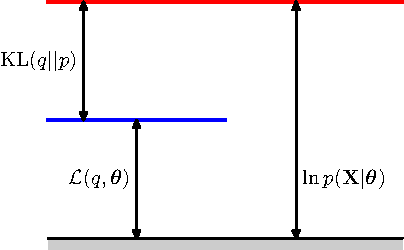
\includegraphics[width=0.85\textwidth]{kld1.pdf}
	\caption{KL散度}
	\label{kld1}
\end{figure}


\begin{remark}
现在我们讨论的是离散的情形, 对于连续情形可类似讨论, 比如假设$q(\bm{Z})$为连续分布, 则有
\begin{align*}
\ln p(\bm{X} | \bm{\theta}) & = \ln \frac{p(\bm{X}, \bm{Z} | \bm{\theta})}{p(\bm{Z} | \bm{X}, \bm{\theta})}  = \int q(\bm{Z}) \ln \frac{p(\bm{X}, \bm{Z} | \bm{\theta})}{p(\bm{Z} | \bm{X}, \bm{\theta})} \diff \bm{Z} \\
& = \int q(\bm{Z}) \ln \left( \frac{p(\bm{X}, \bm{Z} | \bm{\theta})}{p(\bm{Z} | \bm{X}, \bm{\theta})} \cdot \frac{q(\bm{Z})}{q(\bm{Z})} \right) \diff \bm{Z} \\
& = \int q(\bm{Z}) \left( \ln \frac{q(\bm{Z})}{p(\bm{Z} | \bm{X}, \bm{\theta})} + \ln \frac{p(\bm{X}, \bm{Z} | \bm{\theta})}{q(\bm{Z})} \right) \diff \bm{Z} \\
& = \int q(\bm{Z}) \cdot \ln \frac{q(\bm{Z})}{p(\bm{Z} | \bm{X}, \bm{\theta})} \diff \bm{Z} + \int q(\bm{Z}) \cdot \ln \frac{p(\bm{X}, \bm{Z} | \bm{\theta})}{q(\bm{Z})} \diff \bm{Z} \\
& = - \int q(\bm{Z}) \cdot \ln \frac{p(\bm{Z} | \bm{X}, \bm{\theta})}{q(\bm{Z})} \diff \bm{Z} + \int q(\bm{Z}) \cdot \ln \frac{p(\bm{X}, \bm{Z} | \bm{\theta})}{q(\bm{Z})} \diff \bm{Z} \\
& = \mathrm{KL}(q||p) +  \mathcal{L}(q,\bm{\theta})
\end{align*}

\end{remark}


现在考虑 EM 算法的迭代过程.

记上一次迭代得出的参数为$\bm{\theta}^{\mathrm{old}}$, 现在我们选取$q(\bm{Z})$使得$\mathcal{L}(q, \bm{\theta}^{\mathrm{old}})$最大化, 由于此时$\ln p(\bm{X} | \bm{\theta}^{\mathrm{old}})$并不依赖于$q(\bm{Z})$, 相当于一个定值, 也即$\mathcal{L}(q, \bm{\theta}^{\mathrm{old}})$的上限(在$\bm{\theta}^{\mathrm{old}}$固定的时候)是一个定值, 因此它取得最大值的条件就是$\mathrm{KL}(q || p) = 0$, 这等价于$q(\bm{Z}) = p(\bm{Z} | \bm{X}, \bm{\theta}^{\mathrm{old}})$, 将其代入到$\mathcal{L}(q, \bm{\theta}^{\mathrm{old}})$的表达式中可以得到
\begin{align*}
\mathcal{L} (q, \bm{\theta}) & = \sum_{\bm{Z}} p(\bm{Z} | \bm{X}, \bm{\theta}^{\mathrm{old}}) \ln p(\bm{X}, \bm{Z} | \bm{\theta}) - \sum_{\bm{Z}} p(\bm{Z} | \bm{X}, \bm{\theta}^{\mathrm{old}}) \ln p(\bm{Z} | \bm{X}, \bm{\theta}^{\mathrm{old}}) \\ 
& = \mathcal{Q}(\bm{\theta}, \bm{\theta}^{\mathrm{old}}) + \mathrm{const}
\end{align*}

其中 const 是常量, 而$\mathcal{Q}(\bm{\theta}, \bm{\theta}^{\mathrm{old}})$则正是我们之前所得到的同时包含了样本和隐变量的对数似然函数关于隐变量的期望, 因此这一步对应于EM算法中的E步.
\begin{figure}[!htb]
	\centering
	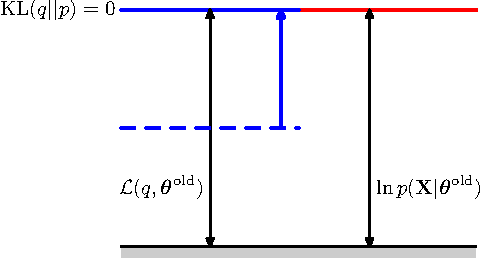
\includegraphics[width=0.85\textwidth]{kld2.pdf}
	\caption{E步}
	\label{kld2}
\end{figure}

在接下来的 M 步中, 我们是固定住分布$q(\bm{Z})$, 再选取合适的$\bm{\theta}^{\mathrm{new}}$使$\mathcal{L}(q, \bm{\theta})$最大化, 这次其上界$\ln p(\bm{X} | \bm{\theta})$也依赖于变量$\bm{\theta}$, 并会随着$\mathcal{L}(q, \bm{\theta})$的增大而增大. 一般情况下$\ln p(\bm{X} | \bm{\theta})$增大的量会比$\mathcal{L}(q, \bm{\theta})$要多一些, 这时候 KL 散度那一项在新的参数$\bm{\theta}^{\mathrm{new}}$下又不为零了, 因此我们可以进入下一轮迭代, 重新回到 E 步去求新的$q(\bm{Z})$; 另一方面, 如果 KL 散度那一项在新的参数$\bm{\theta}^{\mathrm{new}}$下还是等于$0$, 那么说明参数$\bm{\theta}$的值已经几乎不变了, 也就是说迭代收敛到一个(至少是局部的)最优解了, 我们的迭代过程可以结束了.
\begin{figure}[!htb]
	\centering
	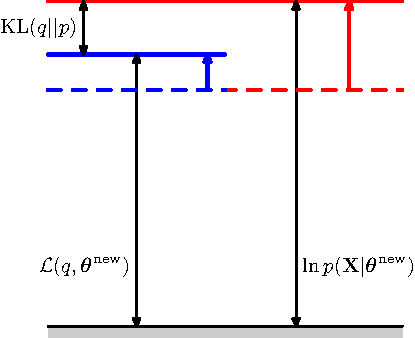
\includegraphics[width=0.85\textwidth]{kld3.pdf}
	\caption{M步}
	\label{kld3}
\end{figure}

在上面的推导中我们可以看到, 每一次迭代 E 步和 M 步两个步骤都是在对解进行改进, 因此迭代的过程中得到的似然函数会逐渐逼近(至少是局部的)最优值, 因此结果肯定是会收敛的.

以上便是 EM 算法背后的原理. 此外, 也可参考 Andrew Ng 的讲义, 该讲义对 EM 算法的原理也解释的很好.






\section{总结}
\subsection{参考资料}
\begin{enumerate}[(1)]
\item 概率论与数理统计课本:

本文的第一个一维的那个例子来自于课本, 以及最大似然估计的回顾也来自于课本.

\item 数据分析方法课本:

重点看最后一章贝叶斯统计的部分, 虽然只有短短的一章, 但是知识衔接的很好(知识最好有一个衔接的体系, 这样才能融会贯通).

\item \url{http://blog.csdn.net/zouxy09/article/details/8537620}: CSDN上的一篇博客, 本文身高的例子来自于此, 解释的比较通俗易懂.

\item \url{http://blog.pluskid.org/?p=39}: pluskid的博客, 介绍了高斯混合模型, 以及这篇 EM 算法 \url{http://blog.pluskid.org/?p=81}, 本文大部分内容也来源于此, pluskid 的博客写的很不错.

\item \url{https://en.wikipedia.org/wiki/Jensen%27s_inequality}: 关于 Jensen 不等式的内容, 对于 Jensen 不等式作了完整介绍, 并且顺带证明了 KL 散度的非负性, 另可参见 \url{https://zh.wikipedia.org/wiki/%E5%90%89%E5%B8%83%E6%96%AF%E4%B8%8D%E7%AD%89%E5%BC%8F}和 \url{https://zh.wikipedia.org/wiki/%E7%9B%B8%E5%AF%B9%E7%86%B5}.

\item PRML: 这个不多说了, 关于 KL 散度的引入以及第二章对多元高斯分布的参数估计.

\item Andrew Ng 的 EM 算法的讲义: 在本地电脑中, 本文几乎没有介绍, 但非常值得一看.

\end{enumerate}



\subsection{混合高斯模型的应用场景}
混合高斯高斯模型主要可用于聚类, sklearn (\url{http://scikit-learn.org/stable/modules/generated/sklearn.mixture.GMM.html}) 和 R 的 mixtools 包 (\url{https://www.r-bloggers.com/fitting-mixture-distributions-with-the-r-package-mixtools/}) 都有相关函数.

关于二维数据的例子比较多, 对于一维数据, 有几个图也展示的不错, 比如 \url{http://www.science-emergence.com/Articles/Mod%C3%A8le-de-m%C3%A9langes-gaussiens-GMM-1d-avec-python/} 和 \url{http://www.astroml.org/book_figures/chapter4/fig_GMM_1D.html}, 这两个是用借助 sklearn 画的, 还有 \url{http://tinyheero.github.io/2016/01/03/gmm-em.html}, 这个是用 R 画的.




\subsection{混合高斯模型的优缺点}



\subsection{EM 算法的应用场景}








\newpage

\section*{附录}










\end{document}